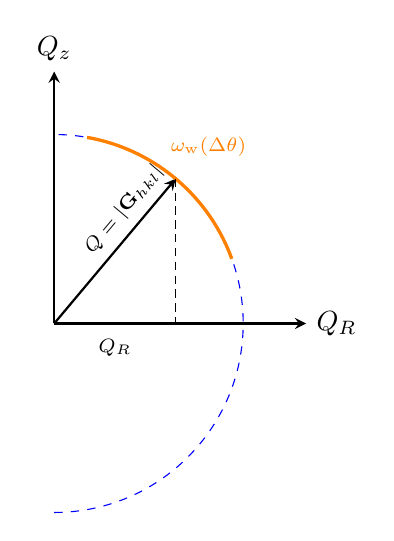
\begin{tikzpicture}[scale=2,>=stealth]
  \def\R{1.2}        % Bragg-sphere radius
  \def\Raxis{1.6}    % axis length
  \def\angleMid{50}  % midpoint angle of mosaic arc (degrees)

  % Folded Bragg locus in the radial coordinate Q_R >= 0
  \draw[dashed,blue] (0,-\R) arc (-90:90:\R);

  % reciprocal-space axes
  \draw[->,thick] (0,0) -- (0,\Raxis) node[above] {$Q_z$};
  \draw[->,thick] (0,0) -- (\Raxis,0) node[right] {$Q_R$};

  % radius vector at midpoint of mosaic arc, label closer to tip
  \coordinate (Gvec) at ({\R*cos(\angleMid)},{\R*sin(\angleMid)});
  \draw[thick,->] (0,0) -- (Gvec)
       node[pos=0.7, above, sloped] {\scriptsize $Q=|\mathbf G_{hkl}|$};

  % mosaic arc on the Bragg sphere, labeled with omega(theta)
  \draw[very thick,orange]
    ({\R*cos(20)},{\R*sin(20)}) arc (20:80:\R)
    node[pos=0.6, above right] {\scriptsize $\omega_{\mathrm w}(\Delta\theta)$};

  % projection onto the radial reciprocal-space axis
  \coordinate (Gr) at ({\R*cos(\angleMid)},0);
  \draw[densely dashed] (Gvec) -- (Gr);
  \node[below, yshift = -2pt] at ({0.5*\R*cos(\angleMid)},0) {\scriptsize $Q_R$};

\end{tikzpicture}
